%% monografia.tex, fabiokepler, jeancheiran
%% Copyright 2012-2018 by UNIPAMPA LaTeX group at https://bitbucket.org/unipampaalegrete/monografias-cc-es-repo/
%%
%% This work may be distributed and/or modified under the conditions of the LaTeX Project Public
%% License, either version 1.3 of this license or (at your option) any later version.
%% The latest version of this license is in
%%   http://www.latex-project.org/lppl.txt
%% and version 1.3 or later is part of all distributions of LaTeX version 2005/12/01 or later.
%%
%% Based on the example file abtex2-modelo-trabalho-academico.tex of the abntex2 package
%% (http://abntex2.googlecode.com/) and on the ppgccufmg 1.45beta2 class
%% (http://vilarneto.com/ppgccufmg,
%% http://www.dcc.ufmg.br/pos/alunos/modelodisstese.php
%% and http://www.dcc.ufmg.br/~mirella).
%%
%% Adapted for the Computer Science program at UNIPAMPA (http://www.unipampa.edu.br)
%% by Fabio Kepler (fabio@kepler.pro.br) and Jean Cheiran (jeancheiran@unipampa.edu.br).
%%
%% Version 2.5 - 2018/08
%% Version 2.4 - 2017/05
%% Version 2.3 - 2013/03

% +++++++++++++++++++++++++++++++++++++++++++++++++++++++++++++++++++++++++++++++++++++++++++++++++
% Este modelo utiliza o pacote abnTeX2. Veja como instalá-lo em seu ambiente em
% http://abntex2.googlecode.com/.
% -------------------------------------------------------------------------------------------------
% abnTeX2: Modelo de Trabalho Acadêmico (tese de doutorado, dissertação de
% mestrado e trabalhos monográficos em geral) em conformidade com
% ABNT NBR 14724:2011: Informação e documentação - Trabalhos acadêmicos -
% Apresentação
% -------------------------------------------------------------------------------------------------
% Normas institucionais utilizadas:
% http://porteiras.r.unipampa.edu.br/portais/sisbi/programa-de-capacitacao/
% +++++++++++++++++++++++++++++++++++++++++++++++++++++++++++++++++++++++++++++++++++++++++++++++++

\documentclass[12pt,openright,twoside,a4paper,chapter=TITLE,english]{abntex2}    % frente e verso

% +++++++++++++++++++++++++++++++++++++++++++++++++++++++++++++++++++++++++++++++++++++++++++++++++
% PACOTES
% -------------------------------------------------------------------------------------------------
% Pacotes fundamentais
\usepackage{cmap}           % Mapeamento de caracteres especiais no PDF
\usepackage{lmodern}        % Usa fonte Latin Modern
\usepackage[T1]{fontenc}    % Seleção de codificação de fonte
\usepackage[utf8]{inputenc} % Codificação do arquivo (conversão automática dos acentos)
\usepackage{makeidx}        % Criação de índice
\usepackage[style=abnt,backref=true]{biblatex}
\usepackage{hyperref}       % Formatação do índice
\usepackage{lastpage}       % Usado pela Ficha catalográfica
\usepackage{indentfirst}    % Indenta o primeiro parágrafo de cada seção
\usepackage[usenames,dvipsnames]{xcolor}  % Controle das cores (com nomes)
\usepackage{graphicx}       % Inclusão de gráficos
\usepackage{booktabs}       % Formatação de tabelas
% -------------------------------------------------------------------------------------------------
% Pacotes opcionais
\usepackage{nomencl}        % Para criar uma lista de símbolos
\usepackage{acro}           % Para usar acrônimos e abreviaturas
\usepackage{tikz}           % Para fazer figuras, diagramas e gráficos integrados e elegantes
\usepackage{pgfplots}       % Usa o pacote tikz para fazer gráficos muito melhores que os do Excel
\usepackage{pgfplotstable}  % Para gerar tabelas automaticamente a partir de arquivos com dados
\usepackage{filecontents}   % Para colocar o conteúdo de um arquivo dentro de um arquivo tex
\usepackage{pdfpages}        % Para incluir a folha de aprovação assinada em PDF
\usepackage[olditem]{paralist}       % Listas in-line
\usepackage{colortbl}
\usepackage{multirow}
\usepackage{hhline}
\usepackage[nameinlink]{cleveref}
\usepackage{makecell}
\usepackage{rotating}
% -------------------------------------------------------------------------------------------------
\addto\captionsenglish{% ingles
  %% adjusts names from abnTeX2
  \renewcommand{\folhaderostoname}{Title page}
  \renewcommand{\epigraphname}{Epigraph}
  \renewcommand{\dedicatorianame}{Dedication}
  \renewcommand{\errataname}{Errata sheet}
  \renewcommand{\agradecimentosname}{Acknowledgements}
  \renewcommand{\anexoname}{ANNEX}
  \renewcommand{\anexosname}{Annex}
  \renewcommand{\apendicename}{APPENDIX}
  \renewcommand{\apendicesname}{Appendix}
  \renewcommand{\orientadorname}{Supervisor:}
  \renewcommand{\coorientadorname}{Co-supervisor:}
  \renewcommand{\folhadeaprovacaoname}{Approval}
  \renewcommand{\resumoname}{Resumo} 
  \renewcommand{\listadesiglasname}{List of abbreviations and acronyms}
  \renewcommand{\listadesimbolosname}{List of symbols}
  \renewcommand{\fontename}{Source}
  \renewcommand{\notaname}{Note}
   %% adjusts names used by \autoref
  \renewcommand{\pageautorefname}{page}
  \renewcommand{\chapterautorefname}{Chapter}
  \renewcommand{\figureautorefname}{Figure}
  \renewcommand{\tableautorefname}{Table}
  \renewcommand{\sectionautorefname}{section}
  \renewcommand{\subsectionautorefname}{subsection}
  \renewcommand{\subsubsectionautorefname}{subsubsection}
  \renewcommand{\paragraphautorefname}{subsubsubsection}
  \renewcommand{\imprimirtipotrabalho}{Term Paper }
}

\pgfplotsset{compat=1.18}

% Configurações de aparência do PDF final
%\definecolor{blue}{RGB}{41,5,195}
% \definecolor{webgreen}{rgb}{0,.5,0}
% Metainformações do PDF e cores dos links
\hypersetup{
  portuguese,
  %backref=true,
  %pagebackref=true,
  %bookmarks=true,             % show bookmarks bar?
  %bookmarksnumbered=true,
  bookmarksdepth=4,
  pdftitle={\@title},
  pdfauthor={\@author},
  pdfsubject={\imprimirpreambulo},
  pdfkeywords={UNIPAMPA}{Computação}{UNIPAMPA}{abntex}{TCC},
  %pdfproducer={LaTeX with abnTeX2},     % producer of the document
  pdfcreator={\@author},
  colorlinks=true,           % false: boxed links; true: colored links
  linkcolor=black,            % color of internal links
  citecolor=black,            % color of links to bibliography
  filecolor=black,         % color of file links
  urlcolor=black
}
%   linktocpage,
%   colorlinks,
%   citecolor=webgreen,
%   urlcolor=Maroon,
%   linkcolor=RoyalBlue,
%   filecolor=black,
% -------------------------------------------------------------------------------------------------
% Espaçamentos entre linhas e parágrafos
% O tamanho do parágrafo é dado por
\setlength{\parindent}{1.3cm}
% Controle do espaçamento entre um parágrafo e outro
\setlength{\parskip}{0.2cm} % tente também \onelineskip
% Controles do espaçamento entre linhas
%\OnehalfSpacing       % espaçamento um e meio (padrão);
%\DoubleSpacing        % espaçamento duplo
%\SingleSpacing        % espaçamento simples
% -------------------------------------------------------------------------------------------------
% Para o pacote de acrônimos
\acsetup{make-links} %first-style=short}
% -------------------------------------------------------------------------------------------------
% Para o pacote tikz, pgfplots e pgfplotstable
\usetikzlibrary{arrows,chains,matrix,positioning,decorations.pathreplacing,calc}
% -------------------------------------------------------------------------------------------------
% Para poder usar subfiguras e subtabelas
\newsubfloat{figure}
\newsubfloat{table}
\providecommand*{\subfigureautorefname}{\figureautorefname}
% +++++++++++++++++++++++++++++++++++++++++++++++++++++++++++++++++++++++++++++++++++++++++++++++++


% +++++++++++++++++++++++++++++++++++++++++++++++++++++++++++++++++++++++++++++++++++++++++++++++++
% Informações de dados para CAPA e FOLHA DE ROSTO
% -------------------------------------------------------------------------------------------------
\titulo{Extensionly - A tool for supporting the management of outreach projects and programs in the university: Front-end}
\autor{Lucas Alexandre Fell}
\local{Alegrete}
\data{2022}
\orientador{Prof. Ph.D. Maicon Bernardino da Silveira}
\instituicao{Federal University of Pampa}
%\tipotrabalho{Projeto de Trabalho de Conclusão de Curso~} % Para TCC I
\tipotrabalho{Trabalho de Conclusão de Curso~} % Para TCC II
% O preambulo deve conter o tipo do trabalho, o objetivo, o nome da instituição e a área de concentração
\preambulo{\imprimirtipotrabalho presented in Software Engineering Graduation Course in the Federal University of Pampa as a partial requirement for
obtaining the title of Software Engineering
Bachelor}

\setlength\bibitemsep{1.8\itemsep}
\addbibresource{bibliografia.bib}

\makeindex % Compila o indice
\makenomenclature % Compila a lista de abreviaturas e siglas
% Abreviaturas 
\DeclareAcronym{fig}{
  short = Fig.,
  long  = Figura,
  tag = abreviaturas
}
% Acrônimos/Siglas
\DeclareAcronym{UNIPAMPA}{
  short = Unipampa,
  long  = Federal University of Pampa,
  tag = acronimos
}
\DeclareAcronym{OCA}{
  short = OCA,
  long  = Outreach Curriculum Activity,
  long-plural-form = Outreach Curriculum Activities,
  tag = acronimos
}
\DeclareAcronym{OA}{
  short = OA,
  long  = Outreach Activity,
  long-plural-form = Outreach Activities,
  tag = acronimos
}
\DeclareAcronym{PROEXT}{
  short = PROEXT,
  long  = Dean of Outreach and Culture,
  tag = acronimos
}
\DeclareAcronym{IT}{
  short = IT,
  long  = Information Technology,
  tag = acronimos
}
\DeclareAcronym{MVP}{
  short = MVP,
  long  = Minimum Viable Product,
  tag = acronimos
}
\DeclareAcronym{FORPROEX}{
  short = FORPROEX,
  long  = Forum of Pro-Rectors for Outreach of Brazilian Public Universities,
  tag = acronimos
}
\DeclareAcronym{HEI}{
  short = HEI,
  long  = Higher Education Institution,
  tag = acronimos
}
\DeclareAcronym{HECI}{
  short = HECI,
  long  = Higher Education Community Institution,
  tag = acronimos
}
\DeclareAcronym{SIGAA}{
  short = SIGAA,
  long  = Integrated Academic Activities Management System,
  tag = acronimos
}
\DeclareAcronym{ATE}{
  short = ATE,
  long  = Administrative Technician in Education,
  tag = acronimos
}
\DeclareAcronym{SGCE}{
  short = SGCE,
  long  = Electronic Certificate Management System,
  tag = acronimos
}
\DeclareAcronym{SIPPEE}{
  short = SIPPEE,
  long  = {Information System for Research, Teaching and Outreach Projects},
  tag = acronimos
}
\DeclareAcronym{NGO}{
  short = NGO,
  long  = Non-governmental organization,
  long-plural-form = Non-governmental organizations,
  tag = acronimos
}
\DeclareAcronym{CAEX}{
  short = CAEX,
  long  = Outreach Actions Control,
  tag = acronimos
}
\DeclareAcronym{MoSCoW}{
  short = MoSCoW,
  long  = {Must have, Should have, Could have and Will not have},
  tag = acronimos
}
\DeclareAcronym{API}{
  short = API,
  long  = {Application Programming Interface},
  tag = acronimos
}
\DeclareAcronym{ID}{
  short = ID,
  long  = {Identification},
  tag = acronimos
}
\DeclareAcronym{SAP}{
  short = SAP,
  long  = Academic Project System,
  tag = acronimos
}
\DeclareAcronym{SEI}{
  short = SEI,
  long  = Electronic Information System,
  tag = acronimos
}
\DeclareAcronym{FR}{
  short = FR,
  long  = Functional Requirement,
  tag = acronimos
}

\begin{document}
% Pequenos consertos e ajustes para que fique de acordo com o Manual de Normatização 2011.

\setlength{\ABNTEXsignwidth}{12cm}

%% adjusts names from abnTeX2
% \renewcommand{\folhaderostoname}{Title page}
% \renewcommand{\epigraphname}{Epigraph}
% \renewcommand{\dedicatorianame}{Dedication}
% \renewcommand{\errataname}{Errata sheet}
% \renewcommand{\agradecimentosname}{Acknowledgements}
% \renewcommand{\anexoname}{ANNEX}
% \renewcommand{\anexosname}{Annex}
% \renewcommand{\apendicename}{APPENDIX}
% \renewcommand{\apendicesname}{Appendix}
% \renewcommand{\orientadorname}{Supervisor:}
% \renewcommand{\coorientadorname}{Co-supervisor:}
% \renewcommand{\folhadeaprovacaoname}{Approval}
% % \renewcommand{\resumoname}{Resumo
% % \renewcommand{\englishcontentsname}{Summary}
% % \renewcommand{\englishlistfigurename}{List of figures}
% % \renewcommand{\englishlisttablename}{List of tables}
% % \renewcommand{\englishlistadesiglasname}{List of abbreviations and acronyms}
% \renewcommand{\listadesimbolosname}{List of symbols}
% \renewcommand{\fontename}{Source}
% \renewcommand{\notaname}{Note}
% %% adjusts names used by \autoref
% \renewcommand{\pageautorefname}{page}
% \renewcommand{\sectionautorefname}{section}
% \renewcommand{\subsectionautorefname}{subsection}
% \renewcommand{\subsubsectionautorefname}{subsubsection}
% \renewcommand{\paragraphautorefname}{subsubsubsection}
% \renewcommand{\imprimirtipotrabalho}{Term Paper }

% ---
% Impressão da Capa
\renewcommand{\imprimircapa}{%
  \begin{capa}%
    \center
    {\ABNTEXchapterfont\large\MakeUppercase\imprimirinstituicao}

    \vspace*{\fill}
    {\ABNTEXchapterfont\large\imprimirautor}

    \vspace*{\fill}
    {\ABNTEXchapterfont\bfseries\LARGE\imprimirtitulo}

    \vspace*{\fill}
    ~
    \vspace*{\fill}

    {\large\imprimirlocal}
    \par
    {\large\imprimirdata}

    \vspace*{1cm}
  \end{capa}
}
% ---


% ---
% Impressão da Folha de Rosto
\makeatletter
\renewcommand{\folhaderostocontent}{
  \begin{center}

    {\ABNTEXchapterfont\large\imprimirautor}

    \vspace*{\fill}%\vspace*{\fill}
    {\ABNTEXchapterfont\bfseries\Large\imprimirtitulo}
    \vspace*{\fill}

    \abntex@ifnotempty{\imprimirpreambulo}{%
      \hspace{.45\textwidth}
      \begin{minipage}{.5\textwidth}
        {\SingleSpacing
        \imprimirpreambulo}

        \vspace*{1em}
        \imprimirorientadorRotulo~\imprimirorientador\par

        \abntex@ifnotempty{\imprimircoorientador}{%
          \vspace*{1em}
          \imprimircoorientadorRotulo~\imprimircoorientador%
        }%

      \end{minipage}%
      \vspace*{\fill}
    }%

    {\large\imprimirlocal}
    \par
    {\large\imprimirdata}
    \vspace*{1cm}

  \end{center}
}
\makeatother
% ---

% ---
\renewcommand{\ABNTEXchapterfont}{\rmfamily\bfseries}
\setsecheadstyle{\rmfamily\bfseries}

\renewcommand{\ABNTEXchapterfontsize}{\normalsize}
\renewcommand{\ABNTEXsectionfontsize}{\normalsize}
\renewcommand{\ABNTEXsubsectionfontsize}{\normalsize}
\renewcommand{\ABNTEXsubsubsectionfontsize}{\normalsize}
\renewcommand{\ABNTEXsubsubsubsectionfontsize}{\normalsize}

% Espaçamento entre título e texto
\setlength\afterchapskip{\lineskip}

% Espaçamento entre parágrafos
\setlength{\parskip}{0.cm}

% ---

 % Inclui alguns ajustes finos para que fique de acordo com o Manual de Normatização
\selectlanguage{english}

% ELEMENTOS PRÉ-TEXTUAIS
\imprimircapa % Capa [OBRIGATÓRIO]
\imprimirfolhaderosto % Folha de rosto [OBRIGATÓRIO]

% -----------------------------------------------
% Folha de aprovação [OBRIGATÓRIO]
% -----------------------------------------------
% Este é um exemplo de Folha de aprovação, elemento obrigatório da NBR 14724/2011 (seção 4.2.1.3).
% Você pode utilizar este modelo até a aprovação do trabalho.
% Após isso, altere o conteúdo deste arquivo para inserir uma imagem da página assinada pela banca usando
% o modelo que está no final deste arquivo.

% -----------------------------------------------
% Folha de aprovação antes da defesa do TCC
% -----------------------------------------------
%\begin{comment}
\begin{folhadeaprovacao}
  \begin{center}
    {\ABNTEXchapterfont\large\imprimirautor}

    \vspace*{\fill}%\vspace*{\fill}
    {\ABNTEXchapterfont\bfseries\Large\imprimirtitulo}
    \vspace*{\fill}

    \hspace{.45\textwidth}
    \begin{minipage}{.5\textwidth}
      \imprimirpreambulo
    \end{minipage}%
    \vspace*{\fill}
  \end{center}

  \begin{center}
    \imprimirtipotrabalho presented and approved on ..... .............. of ......

    Committee members:
  \end{center}

  \assinatura{\textbf{\imprimirorientador} \\ Supervisor \\ UNIPAMPA}
  \makeatletter
  \abntex@ifnotempty{\imprimircoorientador}{%
    \assinatura{\textbf{\imprimircoorientador} \\ Coorientador \\ <sigla da instituição>}%
  }
  \makeatother
  \assinatura{\textbf{Prof. Ph.D. Amanda Meincke Melo} \\ UNIPAMPA}
  \assinatura{\textbf{Prof. Ph.D. Williamson Alison Freitas Silva} \\ UNIPAMPA}

\end{folhadeaprovacao}
%\end{comment}
% -----------------------------------------------
% Folha de aprovação após a defesa do TCC com a imagem da folha de aprovação assinada pela banca.
% -----------------------------------------------
\begin{comment}
\begin{folhadeaprovacao}

  % Escolher entre uma das seguintes opções para inclusão da folha de aprovação
  % Versão assinada em arquivo PDF (incluir no arquivo principal o comando \usepackage{pdfpages})
  %\includepdf{pretextuais/aprovacao.pdf}

  % Ou, versão assinada em arquivo de imagem (jpg, png, etc)
  % Mas prefira em PDF. Em imagem é preciso acertar os recuos das margens:
  %\vspace*{-4cm}
  %\hspace*{-3.5cm}
  %\includegraphics[width=\paperwidth]{pretextuais/aprovacao}

\end{folhadeaprovacao}
\end{comment}
 % Folha de aprovação [OBRIGATÓRIO]
\begin{dedicatoria}
   \vspace*{\fill}
   \begin{flushright}
     This work is dedicated to all software engineering empiricists who,\\
     at some point, felt like giving up\\
     and throwing everything up in the air,\\
     but still made it to the end.
   \end{flushright}
   \vspace*{\fill}
\end{dedicatoria}
 % Dedicatória [OPCIONAL]
\begin{agradecimentos}

  I would like to thank my family, Isabel, Marco and Maitê for their unbounded love and support. I wouldn't be here without their help throughout the years and the education they were able to provide me. For that, I will be always grateful.

  I am also thankful for the knowledge and education I received from each of my professors during my time at the University. This work wouldn't be possible without them. College has been a challenge since the start, especially during the COVID pandemic, but thanks only to their patience and effort in teaching, that was I able to reach this far in the course.

  My advisor, Maicon Bernardino, for motivating, guiding, and being a great supervisor. For without his help and patience, this whole study could've been much more difficult than it needs to be.

  My friend and roommate throughout the college years, Igor, for the bond we created through college that I'm sure will last for many years to come. Also, thanks for all the discussions and knowledge sharing we've had during each discipline of the course. It would've been much, much harder to come this far without his help.

\end{agradecimentos} % Agradecimentos [OPCIONAL]
\begin{epigrafe}
  \vspace*{\fill}
	\begin{flushright}
		\textit{``The most beautiful experience we can have is the mysterious.\\
		It is the fundamental emotion that stands at the cradle of true art and true science.''
		(Albert Einstein)}
	\end{flushright}
\end{epigrafe}
 % Epígrafe [OPCIONAL]
\begin{resumo}
  Em 2023, o processo de curricularização de novas Ações de Extensão será implantado obrigatoriamente pelas Instituições de Ensino Superior do país. Apesar disso, em sua maioria, as Instituições não possuem um processo completamente automatizado para a gestão dos Programas e Projetos de Extensão, que continuaria sendo realizada manualmente pelo coordenador ou colaboradores de extensão. A realidade não é diferente na \acs{UNIPAMPA}, onde foi inicialmente identificada essa oportunidade de melhoria no processo. Essa é a motivação principal por trás da Extensionly. Desenvolver uma solução que contemple todos os processos envolvidos no ciclo de vida das atividades extensionistas. Para isso, o esforço conjunto de dois autores tem sido realizado, tanto na geração de artefatos de suporte à pesquisa, como no desenvolvimento da solução. Este trabalho tem como foco principal a parte do \textit{front-end} e experiência de usuário do sistema, enquanto que o outro concentra-se no \textit{back-end} da aplicação. Sobre os artefatos gerados, foram eles:
  \begin{inparaenum}[(a)]
    \item Um protocolo, formulado e executado para a realização de uma revisão sistemática na literatura cinza, de acordo com as diretrizes da Engenharia de Software, com o objetivo de encontrar ferramentas similares. Os resultados foram classificados e, a partir de sua análise, foi realizada uma extração de requisitos e necessidades iniciais da aplicação;
    \item Um \textit{survey}, cuja confecção foi realizada segundo definições e diretrizes encontradas na literatura. Esse estudo foi direcionado à comunidade acadêmica da \ac{UNIPAMPA} e teve como objetivo classificar, escala de importância, os requisitos previamente coletados com a revisão na literatura cinza. Os resultados foram analisados e, a partir deles, iniciou-se o desenvolvimento da solução proposta, uma solução \textit{web} para apoiar o processo de gestão dos programas e projetos de de extensão, cujos benefícios serão principalmente a redução de esforço necessário para a criação de uma atividade extensionista e a agilidade no engajamento dos extensionistas voluntários.
  \end{inparaenum}

  \vspace{\onelineskip}

  \noindent
  \textbf{Palavras-chave}: Ferramenta. Survey. Literatura Cinza. Front end. Extensão. Universidade.
\end{resumo}
 % Resumo [OBRIGATÓRIO]
\begin{resumo}[Abstract]
  In 2023, the process of curricularization of new outreach actions will be implemented by the country's \ac{HEI}. Nevertheless, the Institutions do not have a completely automated process for the management of outreach programs and projects, which would continue to be carried out manually by the coordinator or outreach collaborators. Reality is no different in \acs{UNIPAMPA}, where this opportunity for improvement of the process was initially identified. This is the main motivation behind Extensionly. To develop a solution that contemplates all processes involved in the life cycle of outreach activities. For this, the joint effort of two authors has been made, both in the generation of research support artifacts and in developing the solution. This work has as its main focus in the front end and system user experience, while the other focuses on the application back end. About the artifacts generated, they were as follows:
  \begin{inparaenum}[(a)]
    \item A protocol, formulated and executed to perform a systematic review in grey literature, according to the software engineering guidelines, with the objective of finding similar tools. The results were classified and, from their analysis, an extraction of initial requirements and needs of the application was performed;
    \item A survey, whose confection was performed according to definitions and guidelines found in the literature. This study was directed to the academic community of \acs{UNIPAMPA} and aimed to classify, in the scale of importance, the requirements previously collected with the review in grey literature. The results were analyzed and, from them, the development of the proposed tool will start: A web solution to support the management of outreach programs and projects, whose benefits will be mainly the reduction of effort needed to create an outreach activity and agility in the engagement of volunteer outreach participants.
  \end{inparaenum}

  \vspace{\onelineskip}

  \noindent
  \textbf{Key-words}: Tool. Survey. Grey Literature. Front end. Outreach Activities. University.
\end{resumo}
 % Abstract (resumo em inglês) [OBRIGATÓRIO]
% Figuras/Ilustrações [OPCIONAL]
\pdfbookmark[0]{\listfigurename}{lof}
\listoffigures*
\cleardoublepage

% Tabelas [OPCIONAL]
\pdfbookmark[0]{\listtablename}{lot}
\listoftables*
\cleardoublepage

% Siglas [OPCIONAL] (veja o pacote acro e os exemplo acima)
\pdfbookmark[0]{\listadesiglasname}{loa}
\printacronyms[include=acronimos,name=\listadesiglasname,heading=chapter*]
\cleardoublepage

% Sumário
\pdfbookmark[0]{Table of contents}{toc}
\tableofcontents*
\cleardoublepage

\textual

% Introdução - descrever projeto em cooperação (front/back), extenso e feito em 2 mãos, estabelecer limites
% Motivação - SAP (unipampa), gestão da extensão, inexistência da gestão do projeto no sistema (emissão de certificados...) 
%=========================================
\chapter{Introduction}\label{introduction}
%=========================================

This work is part of a collaborative effort by two students from the Software Engineering course. Since the complexity and size of the problem were bigger than what the academy is used to seeing on \acp{TP}, the work was split among both authors. This decision was supported and previously agreed upon by their supervisor.

The effort was separated as follows: While this paper encompasses all of the front-end system requirements, such as analytics, multiple languages, component styling, design of the pages with the user interface and user experience, the counterpart focuses heavily on the back-end system requirements. Both projects are going to be separate implementations, will live in different version control repositories and both will have their own specific DevOps pipelines and deployments.

The \acl{UNIPAMPA} provides a number of options for students to engage in environments outside of the institution. An outreach activity can be defined as the following, in accordance with the 317th CONSUNI Resolution from April 29, 2021: An action that integrates the curriculum matrix and the organization of research, constituting an interdisciplinary, political, educational, cultural, scientific, and technological process \citeonline{res317}. Additionally, it fosters the development and use of knowledge in constant articulation with teaching and research, which transforms the interaction between \ac{UNIPAMPA} and society.

There are four (4) different modalities for outreach activities \citeonline{res317}:
\begin{inparaenum}[(i)]
  \item Program: a series of actions with a medium to long-term time frame that are focused on a single goal;
  \item Project: it is typically associated with a Program and has a clear goal and a set duration;
  \item Course: training activity, with short duration, and;
  \item Event: an action with an artistic, cultural and scientific character, with a well-defined duration.
\end{inparaenum}

As an illustration, consider the JEDI Program, which enlists the help of the local community (both academic and non-academic) as well as public or private businesses to address local issues and promote capacity building and IT training \cite{chamadaJedi}.

To register a new \ac{OA}, it is first necessary to identify whether it is a Specific or Linked \ac{OA} - whether it is linked to an Undergraduate Curriculum Component or not. The \ac{OA} insertion process is carried out at the \ac{PROEXT} of \ac{UNIPAMPA}. Once registered, the course committee will need to appoint one or more professors as outreach supervisors \cite{res317}.

The supervisor's duties also include creating and disseminating a biannual report detailing the outreach efforts conducted during the course, validating the use of Specific \acp{OA}, and evaluating the formative character of the action carried out by the student.

The student is responsible for requesting the use and validation of the hours spent in the activity with the Academic Secretary of the course after contacting the supervisor and expressing interest in an \ac{OA} \cite{res317}. Additionally, the professor is in charge of choosing and enrolling any student who expresses interest in the \ac{OA} program up until there are openings.

\section{Motivation}\label{sec:motivation}

It should come as no surprise that time is crucial in the academic setting. Because it is such a valuable resource, it needs to be handled with extreme caution. As there is currently no solution to handle all the requirements of generating and administering outreach programs in \ac{UNIPAMPA}, time is what propels this initiative forward.

The process of curricularization of the new \ac{OA} will be mandatedly implemented by \ac{HEI} in Brazil starting in 2023 as a result of Res. No317 \cite{res317}. However, the coordinator or other team members of the Outreach Programs and Projects would handle all management manually. In light of this, a number of problems with this manual method were found that might be easily resolved by adding a tool to assist the management process.

This implies that the professors and coordinators must personally complete everything, including constructing a project, submitting and getting it authorized, sending emails and making registration forms to open it for the students to join and eventually earn their participation certificate. Given the numerous emails the student receives from the institution each day, it is possible that one or more of the offers will go overlooked. The entire process is not optimized and requires a lot of time and work to complete.

Also due to the institutional program ``Unipampa Cidadã'' (Unipampa Citizen) - which aims to dedicate a portion of the hours currently invested in outreach activities in projects and areas of great social relevance - it is expected that the enrollment rate of new students in higher education will increase \cite{unipampacidada}, which consequently highlights even more the importance of automating manual processes at the university.

\section{Research Aims and Objectives}\label{sec:objectives}

According to what has been presented, this \ac{TP} has the research aim of developing the front-end part of a tool in which all the current management of \acp{OA} will be carefully observed and reproduced, in order to reduce the effort of the professors and supervisors with the manual steps of the process.

In order to achieve this, the following research objectives were defined:

\begin{itemize}
  \item Systematically review grey literature works and products in order to find similar solutions, collecting the first batch of requirements.
  \item Elaborate a survey, according to \citeonline{kasunic2005designing}, in order to discover new system requirements and in order to better understand the target users' needs.
  \item Analyze the results and refine the elicited requirements to create tangible tasks and an implementation roadmap.
  \item Study current market technologies, programming languages and frameworks to build a stack which delivers a great user experience and is creates a codebase that is easily maintained.
  \item Create a working \ac{MVP} of the system which implements at first the most critical collected and refined requirements for the system to become usable by early users to provide feedback for the product's further development \cite{becker_2020}.
\end{itemize}

\Cref{tbl:intro-objectives} also describes the research aim and questions.

\begin{table}[!htb]
  \centering
  \caption{Synthesis of the Research Aim and Research Objectives.}
  \label{tbl:intro-objectives}
  \footnotesize
  \begin{tabular}{l|p{11cm}}
    \bottomrule
    \rowcolor[rgb]{0.749,0.749,0.749} \multicolumn{1}{c|}{\textbf{Topic}}                  & \multicolumn{1}{c}{\textbf{Description}}                                                                                                                                                                                              \\
    \hline
    \rowcolor[rgb]{0.898,0.898,0.898} \textcolor[rgb]{0.145,0.145,0.145}{\textbf{Subject}} & Management of outreach programs and projects.                                                                                                                                                                                         \\
    \textbf{Study}                                                                         & Tool for Support in management of outreach programs and projects.                                                                                                                                                                     \\
    \rowcolor[rgb]{0.898,0.898,0.898} \textbf{Research Question}                           & How can a tool to support the management of outreach programs and projects of \acs{UNIPAMPA} optimize the management of proposition, registration, dissemination and accountability processes of outreach actions?                    \\
    \textcolor[rgb]{0.145,0.145,0.145}{\textbf{Research Hypothesis}}                       & With a tool to support the management of outreach programs and projects, it is possible to have a reduction on the effort needed to create an outreach activity and an increase in the engagement of volunteer outreach participants. \\
    \rowcolor[rgb]{0.898,0.898,0.898} \textbf{Research Aim}                                & Develop the front end of a tool to support the management of outreach programs and projects of \acs{UNIPAMPA}                                                                                                                         \\
    \textbf{Research Objectives}                                                           & Report results and execution methods of the following processes:
    \begin{inparaenum}[(i)]
      \item Research: Analyze similar tools, state the processes that will be made available by the tool, conduct surveys with the organizers and participants of \acp{OA}, understand the limitations of current processes.
      \item Planning: Elicitate functional and non functional requirements, identify stakeholders, define architecture and technologies.
      \item Development: Elaborate the features defined, build the entire front end.
      \item Deployment: Perform experiments with possible end users, collect feedback and implement appropriate improvements and corrections.
    \end{inparaenum}                                                                                                          \\
    \toprule
  \end{tabular}
  \fonte{Author.}
\end{table}

\section{Contribution}\label{sec:contribution}

The main contribution of this study will be the implementation of an \ac{MVP}, in the form of a web application, to support and automate the whole process of \acp{OA} in the university. It also aims to generate valuable artifacts about the state of outreach activities management tooling and support in Brazil, such as a grey literature review. A survey is also conducted, aiming to better understand the needs of outreach participants regarding this specific kind of tooling. Due to the complexity of this proposal, as previously mentioned, the effort was split amongst two \acp{TP}. This one focuses on the development of a web app, with all its related challenges, but it doesn't encompasses the back-end services in detail.

As for the artifacts generated to support the research, such as the grey literature systematic review and the survey, all of them were done in conjunction by both authors and are not related specifically to a single work. The other author is Igor Dalepiane da Costa.

\section{Organization}\label{sec:organization}

This document is organized according the following chapters:

\begin{itemize}
  \item \textbf{Chapter 2: Methodology}: Describes how the study was planned, the adopted methodology and the approaches used to conduct it.
  \item \textbf{Chapter 3: Background}: Important information and details of concepts related to the study, e.g. outreach activities in Brazil and in the \acl{UNIPAMPA}, federal laws and similar tools.
  \item \textbf{Chapter 4: Grey Literature}: How the protocol was structured, results, discovered tools, preliminary requirements.
  \item \textbf{Chapter 5: Survey}: How it was structured, results, validation of refined requirements with the target audience.
  \item \textbf{Chapter 6: Extensionly}: Revolves around implementation details, created artifacts, technologies used, the software engineering process, DevOps practices and the incorporation of analytics.
\end{itemize}
 % [OBRIGATORIO]
% Metodologia 3-4 pags, desenho da pesquisa (bpmn) com fases, atividades, cronograma desde o anteprojeto
%=======================================
\chapter{Methodology}\label{methodology}
%=======================================

This chapter discusses how the study was planned, the adopted methodology and the approaches used to conduct it. The next sections will describe in more detail the procedures and techniques used on the research. Scientific research is described on \Cref{sec:met-1}. In \Cref{sec:met-2}, the research classifications according to \textcite{Prodanov:2013} are defined. After that, in \Cref{sec:met-3}, the research design is shown and explained. A research schedule was created and can be seen in \Cref{sec:met-schedule}. Finally, in \Cref{sec:met-4}, the whole chapter is briefly summarized.

\section{Introduction}\label{sec:met-1}

The word ``Science'' comes from the latin word ``Scire'', which means to learn and to know. For science to be done, there has to be a way to gather new information, building upon what is already known. This is where scientific research fits in. The scientific method, says \textcite{Prodanov:2013}, is a way, through a set of adopted procedures, to achieve knowledge.

It is the basic instrument which turns thoughts into systems, ordering them through procedures, which guides the scientist along the way to achieve his predefined scientific goals. \textcite{Prodanov:2013} also mentions that without the scientific method, there is no science.

\section{Research Classification}\label{sec:met-2}

This research study is defined according to the classification created by \textcite{Prodanov:2013}. It has multiple research types, each of which can be classified into several categories according to the nature, goals, approach and procedures of the study. \Cref{fig:research-classification} shows how the research is categorized. The darker boxes represent categories which apply to this work. The terms in them are described in this section. The other boxes are kept for consistency with the original model.

\begin{figure}[!htb]
  \caption{Research Classification}\label{fig:research-classification}
  \begin{center}
    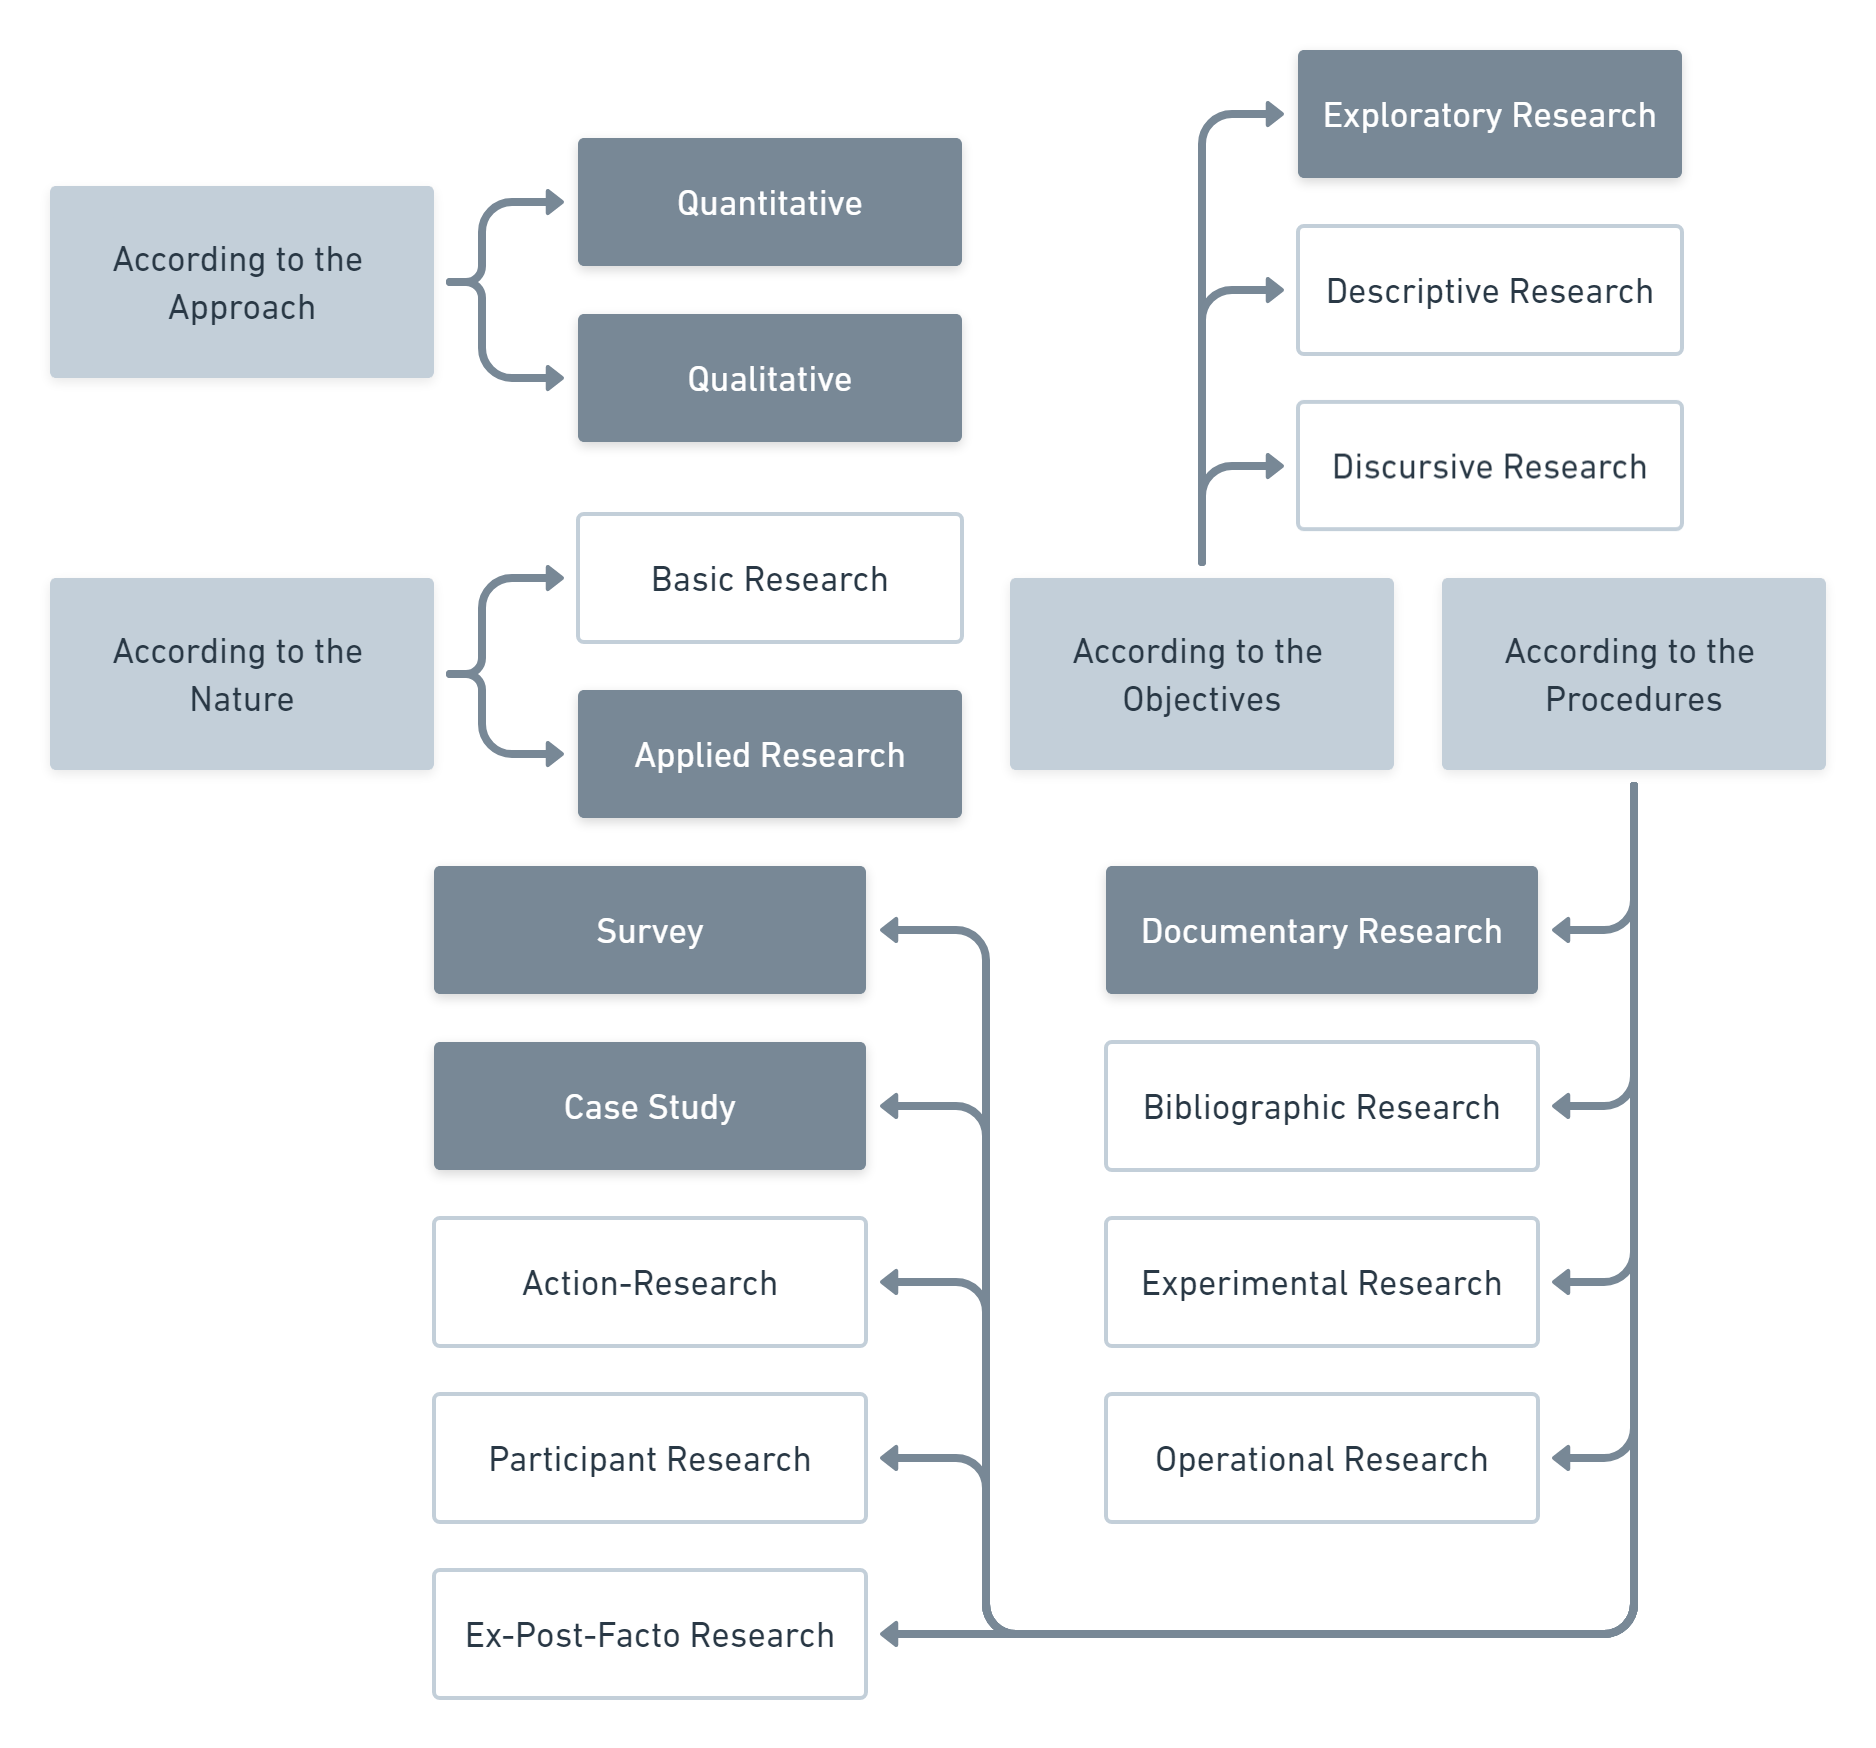
\includegraphics[width=16cm]{img/2-Research Classification@2x.png}
  \end{center}
  \fonte{Adapted from \cite{Prodanov:2013}.}
\end{figure}

Looking through the nature point of view, this is an \textbf{Applied Research}. It has the goal of generating knowledge to the solution of specific problems, through a practical application. It is related to local interests and often has a new process or product as a result.

From the objectives point of view, it is classified as an \textbf{Exploratory Research}, since one of its goals is to discover more information about what is being investigated, and maybe finding a new type of approach to the subject. This type of research generally takes the form of bibliographic research and \textbf{Case Studies}. The former doesn't apply to this study, though, because the final product won't be heavily inspired on white literature. Only the latter applies, because researches of this nature are more focused on the immediate application of knowledge in a circumstantial reality, emphasizing the development of theories.

However, the product will certainly be inspired by grey literature, meaning it fits as a \textbf{Documentary Research}. It is similar to bibliographic research, but the main difference between them is the nature of their sources. While bibliographic research makes fundamental use of contributions from various authors on a given subject, documentary research is based on materials that have not yet received an analytical treatment or that can be reworked according to the research objectives.

According to the technical procedures, this research also features a \textbf{Survey}. They are much more suitable for descriptive rather than explanatory studies. They are inappropriate for the deepening of more complex psychological and psychosocial aspects, but very effective for less delicate problems, for example, electoral preference and consumer behavior. The latter is much more aligned with this study than the former. Surveys are very useful for the study of opinions and attitudes, but little indicated in the study of problems referring to complex social structures. How this technique was applied in the scope of this work is described in detail in \Cref{survey}.

Through the approach point of view, the research is both \textbf{Quantitative}, meaning translating opinions and information into numbers to classify and analyze them. And also \textbf{Qualitative}, because some parts of the study can't be quantified, and must be understood subjectively. An example would be to receive written, detailed feedback from a target-user through the survey.

\section{Research Design}\label{sec:met-3}

In order to conduct the study correctly, a research design was created. The activities are grouped in five phases:
\begin{inparaenum}[(1)]
  \item gather information;
  \item begin development;
  \item write term paper;
  \item develop;
  \item evaluate.
\end{inparaenum}
They are all described in this section and can also be observed in \Cref{fig:research-design}.

\begin{figure}[!htb]
  \caption{Research Design}\label{fig:research-design}
  \begin{center}
    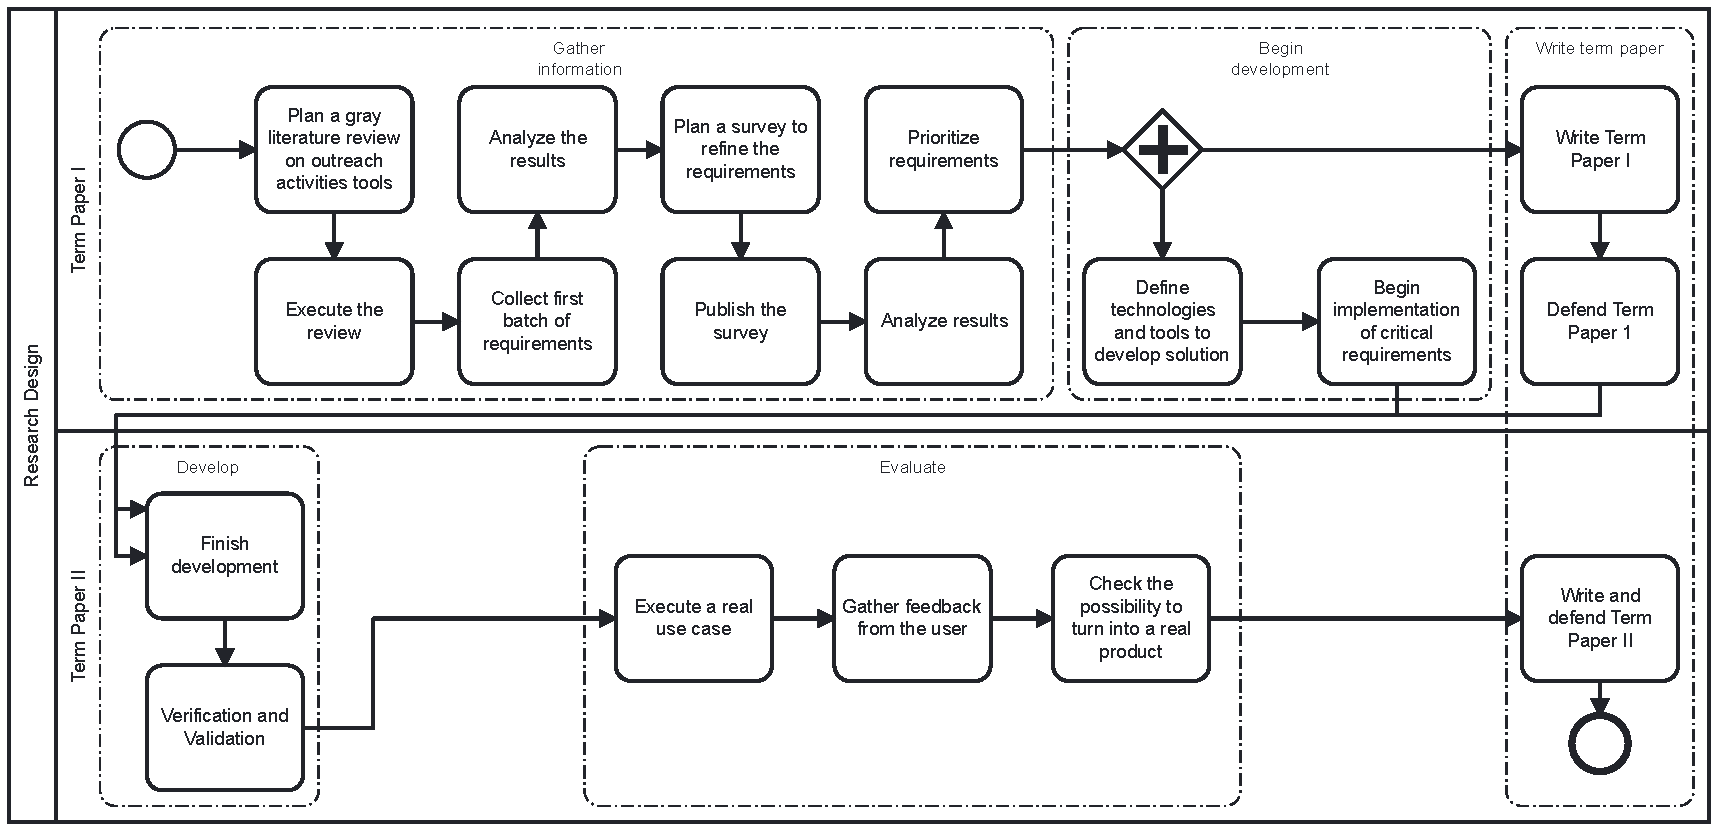
\includegraphics[width=16cm]{img/2-research design.pdf}
  \end{center}
  \fonte{Author.}
\end{figure}

The \textbf{gather information} group aims to create two tangible artifacts: the grey literature systematic review and the survey to better understand the scope of the goal product and most importantly collect a list of well defined requirements.

The \textbf{begin development} group is where the implementation and the term paper writing begins. This is where the technologies used throughout the development of the product are defined. The most important requirements should already be implemented as well.

Next, there is the \textbf{write term paper} group, in which both first and second term papers are going to be written and defended. It is important to notice that the first work will be written while the initial \ac{MVP} implementation is on going.

Continuing to the next milestone, is the \textbf{develop} group, where it is planned to finish the product development. After that, in the \textbf{evaluate} group, is where the real use case will be ran, and the feedback from it, analyzed. If all goes well, the product might turn into a real solution, adopted by the university to be used.

\section{Research Schedule}\label{sec:met-schedule}

In order to have a clear vision of the steps required to run this study, a timeline was created describing what will be done by month until the expected ending of the research. Refer to \Cref{tbl:schedule} for the full overview of what was planned.

\begin{table}[!htb]
  \centering
  \caption{Research Schedule}
  \label{tbl:schedule}
  \scriptsize
  \begin{tabular}{p{4cm}|l|lllll|lll}
    \bottomrule
    \rowcolor[rgb]{0.753,0.753,0.753} \multicolumn{1}{c|}{{\cellcolor[rgb]{0.753,0.753,0.753}}}                                       & \multicolumn{1}{c|}{\textbf{2021/2}} & \multicolumn{5}{c|}{\textbf{2022/1}} & \multicolumn{3}{c|}{\textbf{2022/2}}                                                                                                                                                                                                                                           \\
    \hhline{>{\arrayrulecolor[rgb]{0.753,0.753,0.753}}->{\arrayrulecolor{black}}---------|}
    \rowcolor[rgb]{0.753,0.753,0.753} \multicolumn{1}{c|}{\multirow{-2}{*}{{\cellcolor[rgb]{0.753,0.753,0.753}}\textbf{ Activities}}} & \textbf{Nov - Mar}                   & \multicolumn{1}{c}{\textbf{Apr}}     & \textbf{May}                         & \textbf{Jun}                         & \multicolumn{1}{l}{\textbf{Jul}}     & \textbf{Aug}                         & \textbf{Sep Oct Nov}                 & \textbf{Dec}                         & \multicolumn{1}{c|}{\textbf{Jan}}    \\
    \hline
    \rowcolor[rgb]{0.914,0.914,0.914} Plan and execute systematic review in the grey literature                                       & {\cellcolor[rgb]{0.753,0.753,0.753}} &                                      &                                      &                                      &                                      &                                      &                                      &                                      &                                      \\
    Plan and execute survey with target users                                                                                         &                                      & {\cellcolor[rgb]{0.753,0.753,0.753}} &                                      &                                      &                                      &                                      &                                      &                                      &                                      \\
    \rowcolor[rgb]{0.914,0.914,0.914} Analyze results from previous steps and map requirements                                        &                                      & {\cellcolor[rgb]{0.753,0.753,0.753}} & {\cellcolor[rgb]{0.753,0.753,0.753}} &                                      &                                      &                                      &                                      &                                      &                                      \\
    Plan and start tool development                                                                                                   &                                      &                                      & {\cellcolor[rgb]{0.753,0.753,0.753}} & {\cellcolor[rgb]{0.753,0.753,0.753}} &                                      &                                      &                                      &                                      &                                      \\
    \rowcolor[rgb]{0.914,0.914,0.914} Write Term Paper I                                                                              &                                      &                                      &                                      & {\cellcolor[rgb]{0.753,0.753,0.753}} & {\cellcolor[rgb]{0.753,0.753,0.753}} & {\cellcolor[rgb]{0.753,0.753,0.753}} &                                      &                                      &                                      \\
    Defend Term Paper I                                                                                                               &                                      &                                      &                                      &                                      &                                      & {\cellcolor[rgb]{0.753,0.753,0.753}} &                                      &                                      &                                      \\
    \rowcolor[rgb]{0.914,0.914,0.914} Continue the development of the tool                                                            &                                      &                                      &                                      &                                      &                                      & {\cellcolor[rgb]{0.753,0.753,0.753}} & {\cellcolor[rgb]{0.753,0.753,0.753}} & {\cellcolor[rgb]{0.753,0.753,0.753}} &                                      \\
    Execute a real use case on the tool                                                                                               &                                      &                                      &                                      &                                      &                                      &                                      &                                      & {\cellcolor[rgb]{0.753,0.753,0.753}} &                                      \\
    \rowcolor[rgb]{0.914,0.914,0.914} Write Term Paper II                                                                             &                                      &                                      &                                      &                                      &                                      &                                      &                                      & {\cellcolor[rgb]{0.753,0.753,0.753}} & {\cellcolor[rgb]{0.753,0.753,0.753}} \\
    Defend Term Paper II                                                                                                              &                                      &                                      &                                      &                                      &                                      &                                      &                                      &                                      & {\cellcolor[rgb]{0.753,0.753,0.753}} \\
    \toprule
  \end{tabular}
  \fonte{Author.}
\end{table}

\section{Chapter Summary}\label{sec:met-4}

This chapter provided an idea of how the methodology is defined for the study and how the research can be classified. In addition, the created research design was presented, showcasing the different planned processes for the future and those that have already been executed. \Cref{background} describes all the information and background necessary for the success of this work, while also assisting the reader in better understanding the research methodology previously described. % [OBRIGATORIO]
% Background - extensão universitária no Brasil, curricularização da extensão, soluções/ferramentas de apoio à extensão, leis federais, resoluções unipampa, implantação da extensão, tipos de extensão, perfis de pessoas envolvidas na extensão, programas e projetos de extensão na unipampa
% Unipampa Cidadã
%=====================================
\chapter{Background}\label{background}
%=====================================

In this chapter, information that complement the objective of the study are discussed, helping to understand the policies and resolutions involved. In \Cref{sec:bac-outreach-brazil} the national outreach activity policy will be presented, which is valid for all \acp{HEI} in Brazil. It applies for each \ac{OA} regarding its relation to the academic and external community. Soon after in \Cref{sec:bac-higher-ed} and \Cref{sec:bac-unipampa} the vision of how both the \acp{HECI} as a whole and \acl{UNIPAMPA}, respectively, adapted to receive these new rules is described. Afterwards, in \Cref{sec:bac-programs-projects} the differences between outreach programs and projects will be presented, followed by how new proposals are handled in \Cref{sec:bac-proposals}. Then, a more detailed explanation about the ``\ac{UNIPAMPA} Cidadã'' project is described in \Cref{sec:bac-cidada}. \Cref{sec:bac-tools} showcases current available tools and solutions in the market which are related to the study goal product. Finally in \Cref{sec:bac-summary} a general summary of the chapter is presented.

\section{Outreach activities in Brazil}\label{sec:bac-outreach-brazil}

It is clear that participating in outreach activities has many benefits for the students who decide to take part in it \cite{sellou2011many}. Besides promoting individual growth, the activities can also serve as a bridge connecting students and professors even more. In order to preserve them and encourage younger students to participate in them, the \acl{FORPROEX} (\ac{FORPROEX}), updated the old version of the National Outreach Policy document, published in 1999, with current situations and challenges encountered in recent years. In the new version of the document, \cite{politicaNacional}, some of its objectives are the following:

\begin{itemize}
  \item Achieve the recognition of university outreach activities as an essential tool for the public university.
  \item Ensure that the outreach activity is the solution to any type of social problem faced by the country.
  \item Defend the funding of outreach programs and projects so that they can continue to function.
  \item Promote environmental and sustainable awareness in outreach projects in Brazil.
  \item Promote solidarity both nationally and internationally, covering the area of impact of outreach actions.
\end{itemize}

As a reference for directing and assisting \acp{HECI} to create their outreach policies, \cite{referenciaisPolitica} also highlights the importance of integrating outreach activities with research and teaching, along with discussions of a social nature and the effects of the results on society. The document proposes nine outreach activity types, which are as follows:

\begin{inparaenum}[(1)]
  \item Programs, Projects and Activities for the socialization of knowledge;
  \item Outreach Courses;
  \item Participation in Councils, Academic Events open to the external community: Congresses, Symposia, Seminars, Colloquiums, Course Weeks and related activities;
  \item Promotions of Art, Culture, Sport and Leisure with the involvement of the external community;
  \item Provision of Services, Consultancy and Advisory Services, Technological Extension, Mandatory Internships;
  \item School Clinics;
  \item Curricular Professional Practices;
  \item Course subjects that include practices with external communities;
  \item Research Projects, Course Completion Works,
  Monographs, Dissertations and Theses with methodologies and practices of social intervention with external communities.
\end{inparaenum}

\subsection{\acl{OA} curricularization in Higher Education}\label{sec:bac-higher-ed}

In order to implement what was mentioned above in the \ac{HECI}, the Brazilian Ministry of Education created the Resolution No. 7, of December 18, 2018, which establishes guidelines, principles, foundations and procedures for \acp{OA} in higher education. As such, it was regulated that \acp{OA} will be made available in the form of curricular components for the offered courses \cite{ministerioSuperiorExtensao}.

The document also determines that the outreach activities must comprise at least 10\% (ten percent) of the total student curricular workload of undergraduate courses, and they must also be part of the curriculum of the courses \cite{ministerioSuperiorExtensao}. Another important discussed topic is about the self-assessment of \acp{OA}. The main reason for this is the constant improvement of the activity with teaching, research, student training, teacher qualification, the relationship with society, the participation of partners and other institutional academic dimensions.. This evaluation must include the following:

\begin{inparaenum}[(a)]
  \item How many curricular credits the activity can give;
  \item How it contributes to the Institutional Development Plan and the Pedagogical Projects for the Courses;
  \item The demonstration of the results achieved in relation to the participating public.
\end{inparaenum}

Each \ac{OA} must also contain the planning of its internal activities, the strategies for self-assessment, proposal, development and conclusion. These must be duly recorded and analyzed in order to organize the activity work plans.

As a final note, the \textcite{ministerioSuperiorExtensao} says that the \acp{HEI} will have at most 3 (three) years, counting by the date the document was published, to implement what is being proposed.

\subsection{\acl{OA} curricularization in \acl{UNIPAMPA}}\label{sec:bac-unipampa}

In relation to \ac{UNIPAMPA}, as with other \ac{HECI}, it must create a resolution aimed at standardizing outreach activities in general, presenting what they are, their target audience and their objectives. And thus was born the CONSUNI/UNIPAMPA Resolution No. 332 of 2021, which determines the types of outreach activities, already mentioned earlier in the study, their managing bodies, executing team, possible related processes, and rules such as the minimum duration of 8 (eight) hours \cite{Resolucao-332:2021}.

As \ac{UNIPAMPA} highlights in the Resolution No. 317 of 2021, the main objectives in the insertion of outreach activities in undergraduate courses are the following \textcite{res317}:
\begin{inparaenum}[(i)]
  \item Help students develop their critical, civic, interdisciplinary and responsible education;
  \item Improve teaching in undergraduate courses as a whole and strengthen the inseparability between teaching, research and outreach;
  \item Strengthen \ac{UNIPAMPA}'s social commitment;
  \item Stimulate constructive discussions in all sectors of \ac{UNIPAMPA};
  \item Promote actions that strengthen \ac{UNIPAMPA}'s ethical principles and social commitment in all areas;
  \item Encourage the academic community to be more present in human, academic, social, cultural and economic development.
\end{inparaenum}

\subsection{Outreach Programs and Projects}\label{sec:bac-programs-projects}

According to \textcite{referenciaisPolitica}, Outreach Program and Projects are activities regulated by the institution that articulates events involving teaching and research, always involving the external community. With them students can make decisions directly about the community in which they live, contributing to their evolution and progress.

\textcite{Viero} describes the difference between programs and projects as follows: A project is a set of educative actions of social, cultural or technological nature, with a specific objective and determined deadline. An outreach program is a set of projects, which is preferably multidisciplinary and integrated with research and teaching activities.

A good example of an outreach program is \textcite{JEDI}, which, as mentioned earlier in \Cref{introduction}, aims to solve local problems using technology and involvement with the community. In the first cycle of the program four outreach projects were proposed, each with its own objectives, methodologies and activities:
\begin{inparaenum}[(i)]
  \item Padawan Academy;
  \item Jedi Apprentice;
  \item Jedi Problem-Solving;
  \item Jedi Mind.
\end{inparaenum}

\subsection{Workflow for \acl{OA} Proposals}\label{sec:bac-proposals}

As briefly mentioned in \Cref{sec:bac-unipampa}, \textcite{Resolucao-332:2021} defines a few requirements which must be met before creating new outreach projects or programs. The \acl{UNIPAMPA} created a few workflow visualizations in order to better understand how the process works.

% pedir imagens svg ao igor

In \Cref{fig:outreach-projects-registration}, the registration flow of a new outreach project is presented. It is possible to see that the proposal goes through several steps of corrections and evaluations, being sent to several actors throughout the whole process. Finally, the \acl{PROEXT} is the responsible entity to request final changes or approve the project, granting a new registration number.

\begin{figure}[!htb]
  \caption{Outreach Projects Registration}\label{fig:outreach-projects-registration}
  \begin{center}
    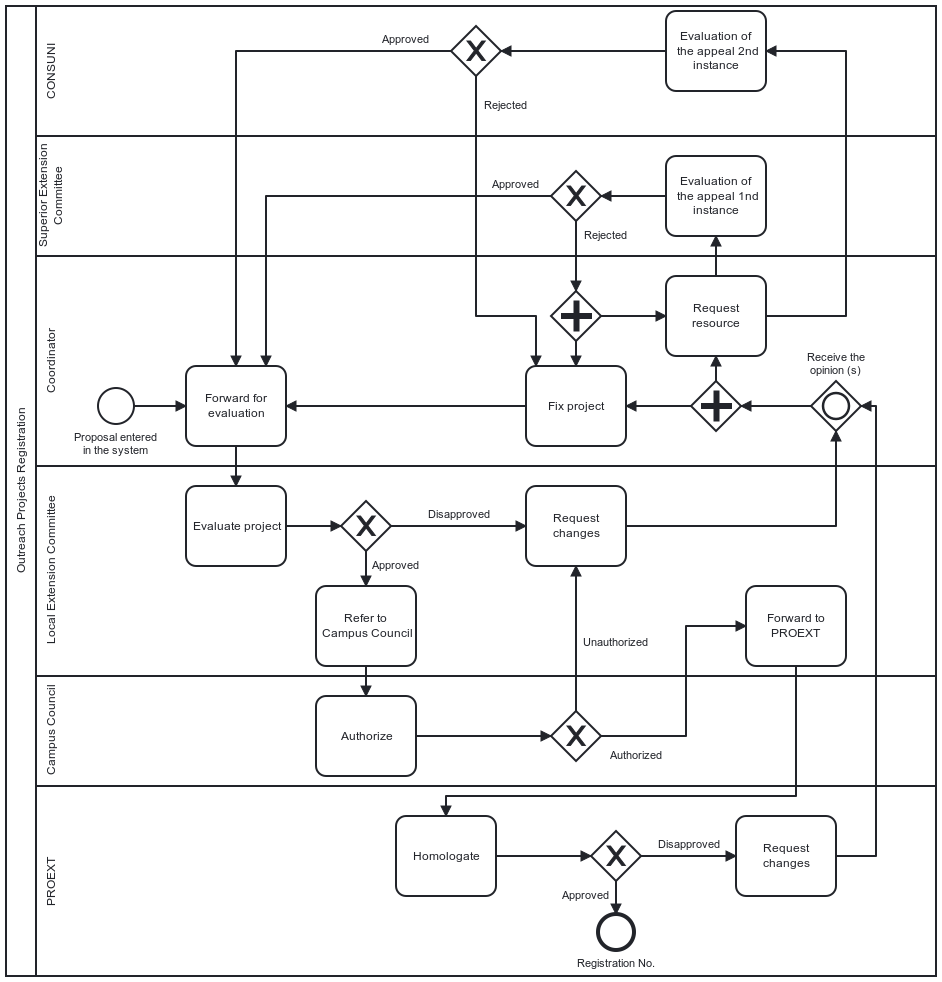
\includegraphics[width=16cm]{img/3-registroDeProjetosDeExtensaoV3.png}
  \end{center}
  \fonte{Adapted from \cite{siteProcessos}.}
\end{figure}

In addition, \Cref{fig:issuance-certificates} presents the steps related to the approval and generation of certificates. Firstly, the proponent of the activity must have the presence list and spreadsheet with information for the generation of certificates. Afterwards, a final report is created and inserted into the \ac{SIPPEE} system. This report is then evaluated and approved, returning to \ac{PROEXT}, who, with the information spreadsheet, sends this data to the \ac{SGCE} system, finally receiving the certificates and sending them to participants' emails.

\begin{figure}[htb]
  \caption{Issuance of Certificates}\label{fig:issuance-certificates}
  \begin{center}
    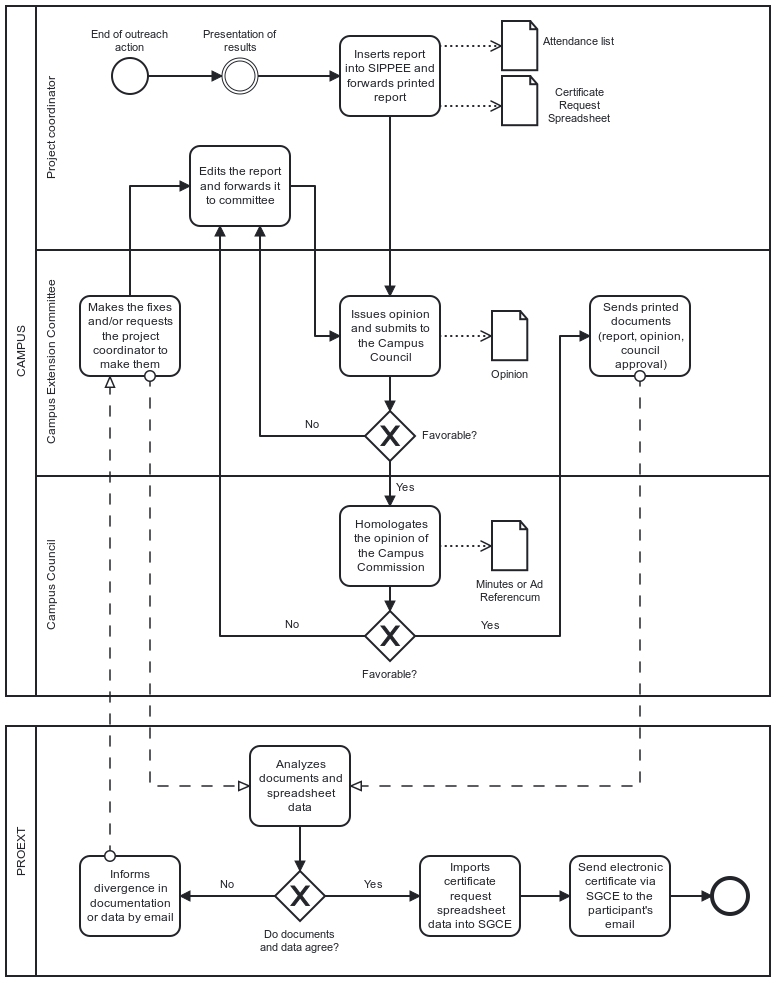
\includegraphics[width=16cm]{img/3-emissaoDeCertificados.png}
  \end{center}
  \fonte{Adapted from \cite{siteProcessos}.}
\end{figure}

\subsection{UNIPAMPA Cidadã}\label{sec:bac-cidada}

The \acl{UNIPAMPA}, through Normative Instruction No. 18 \cite{unipampacidada}, making use of Resolution No. 317, \cite{res317}, establishes the outreach project called ``Unipampa Cidadã'' (Unipampa Citizen). It must be offered by all courses, consisting of citizenship and solidarity activities and with the objective of forming graduates aware of their social responsibility, stimulating and increasing integration with the local community.

After the implementation of the project in the institution's courses, the subject offered for the project must be at least 60 and at most 120 hours, and is required to be taken by all students. The community actions must be carried out in public institutions, \aclp{NGO} and organizations or organized civil society associations. The course outreach supervisor is the one in charge of making the evaluation, planning, monitoring and validation of the project, as well as defining the beginning of the activities.

The project also describes in Normative Instruction No. 18 a form that must be filled when activities are finished. This way, the student will be able to reflect on the impact of the project under his vision, pointing out what he learned during the project's execution. The supervisor can make observations on the student and indicate if he has been approved or not.

\section{Similar Tools}\label{sec:bac-tools}

As \Cref{greyliterature} will later present in more detail the systematic review performed in the grey literature, a research has been done to collect tools related to outreach activities which are available currently in the market. With the results it was possible to list features, details and common points among the tools.

A lot of interesting and different results were found and analyzed, generating artifacts and describing all the cool and unique features each of them had. During the review, the tool that returned the most results and was always present in the search results, was \ac{SIGAA}. However, its scope reaches way beyond just managing outreach activities. It contains features for most processes present in an institution. Another that presented interesting results was \ac{CAEX}, which had several unique features. Overall, it was possible to retrieve ideas of great importance and find inspiration to build a new related product.

\section{Chapter Summary}\label{sec:bac-summary}

This chapter presented guidelines of several resolutions and normatives related to outreach, both in the country as a whole, and in the \acl{UNIPAMPA}. It was also discussed about the similarities and differences between the outreach programs and projects, presenting the most relevant processes involved in their lifecycle. As a recent example of an outreach program, ``Unipampa Cidadã'' (Unipampa Citizen) had part of its objectives and guidelines presented. Finally, it was also discussed a little about the systematic review in the grey literature and the similar tools found. The next chapter aims to discuss more about criteria, methodology, results, research questions, and other relevant information related to the grey literature systematic review.
% Literatura Cinza - protocolo, resultados, lista de ferramentas encontradas -> lista preliminar de requisitos
% Screenshot / análise / resumo sobre 
%==============================================================================
\chapter{Gray Literature}\label{grayliterature}
%==============================================================================
% Survey - lista preliminar da literatura -> validação com usuários reais, agregando novos requisitos
% protocolo, questionário, requisitos propostos, resultados, análise

%==============================================================================
\chapter{Survey}\label{survey}
%==============================================================================

\section{Survey protocol}\label{sec:sv-p}

\subsection{Pilot questionnaire}\label{sec:sv-p:pilot}

As \citeonline[p. 75]{kasunic2005designing} describes, a pilot test is a simulation of the real questionnaire carried out with a small number of members from the target audience. For this, the authors hand picked 7 (seven) people, out of which 4 (four) were students, 2 (two) were professors and 1 (one) was an \acl{TAE} (\ac{TAE}). The reason behind choosing this specific number of respondents is due to the following:
\begin{inparaenum}[(i)]
  \item All defined profiles for the respondents were chosen and
  \item the ratio of 4/2/1 is aligned with the expected numbers of submitted questionnaires per profile.
\end{inparaenum}

Unfortunately, the person chosen for the third profile, \ac{TAE}, wasn't able to answer. However, even though there are 3 (three) profiles, the questionnaire itself only has 2 (two) tracks of questions, one for students and the other for professors/\acp{TAE}. Because of that, the consequences of this happening weren't too impactful.

As for the pilot results, a lot of great feedback was received, along with some compliments on the organization of the questionnaire. There were issues with the person identification section, where the age was changed from a number to a range of numbers, such as between 21-29 years old.

\subsection{Distribute the Questionnaire}\label{sec:survey-distribute}

\section{Threats to validity}\label{sec:sv-validity}

% TAE didn't answer pilot test

\section{Results}\label{sec:sv-results}
% Extensionly - análise e projeto de software, artefatos da implementação, maior capítulo de todos, modelo de domínio, diagrama de componentes, paradigma de programação, tecnologias, processo da engenharia de software, separação frontend/backend (com mais detalhes técnicos), usar figuras e modelos
    % seção devops
    % seção analytics
%==============================================================================
\chapter{Extensionly}\label{extensionly}
%==============================================================================
% Considerações Preliminares - possível publicação em eventos da área, com os resultados encontrados (ERES agosto), mais eventos (SBIE), artigos relacionados à extensão
%==============================================================================
\chapter{Preliminary Considerations}\label{conclusao}
%==============================================================================

% Em Trabalhos de Conclusão de Curso, use ``\emph{Considerações Finais}'' e não ``\emph{Conclusão}''.

% Bom trabalho!

The goal of the current work was to thoroughly examine the administration of \aclp{OA} in order to create a tool that supports the administrative procedures, makes it easier to communicate with the outside world, and improves student participation and dissemination. For this, two artifacts were produced: a review of the gray literature to locate comparable solutions already in use, eliciting their critical features, and a survey of potential end users of the tool to order the requirements by importance and gather additional ideas on the topic.

Five particular goals were established in order to accomplish the overall goal of the work, which is to create the tool's front end to support the management of \ac{UNIPAMPA}'s outreach programs and projects. They were previously described in \Cref{sec:objectives}.

The first goal was to conduct a review of the gray literature to look for features in tools that were similar to what is being proposed. Based on the results, it is clear that this goal was accomplished, as it was possible to identify a number of tools and, in the end, to produce a list of tools that was significant in size, complete with their functionalities and specific information, which was especially helpful in planning.

The second goal relates to the development of a survey to ascertain the viewpoints of potential end users. This goal was accomplished since it was feasible to examine the problems and worries that users had, which made it possible to draw out a number of enhancements and features for the suggested tool.

The third particular goal is the creation of a development roadmap and tangible tasks. This goal was only partially attained because the transition from \ac{FR} to development tasks won't take place until the second phase of this work's development, or \ac{TP} II.

The fourth goal is to research, evaluate, and select a development stack, including a programming language, an architecture, and a framework, for the front end of the suggested tool. This goal was accomplished; prior decisions were presented earlier in \Cref{extensionly}.

The creation of a \ac{MVP} for the tool's front end is the fifth and final specific goal, and it has not yet been accomplished because the tool's development is still on the horizon.

The hypothesis of this work, which can't yet be confirmed or disproved because the application hasn't yet been developed and tested with end users, is that "With a tool to support the management of outreach programs and projects, it's possible to have a reduction on the effort needed to create an outreach activity and an increase in the engagement of volunteer outreach participants." However, given all of the good feedback that the survey respondents supplied, it is extremely probable that this theory will be proven with the accurate and thorough development of the application.

With a tool of this kind, it is feasible to lessen the manual and repetitive work required in the registration of new proposals for outreach efforts, facilitating operations like generating certificates more effectively. This is the research question of this work, described in \Cref{tbl:intro-objectives}. Additionally, students will know where to go if they need assistance with the subject thanks to a platform that centralizes information about university outreach, which will increase the dissemination of new initiatives. With the use of the technology, the connection between the teacher and the participant will also be reinforced, enabling richer interactions and experiences for both parties.

The survey's results gave the researchers insight into what potential end users could think about the presence of a tool like this to help them with related tasks. It allowed for the reevaluation of various implementation-related difficulties while taking into consideration suggestions made. It is safe to state that without a study of these users' opinions, the tool would be in serious danger of not meeting of the previously established expectations.

A lot of effort will be devoted to the application's development for the second iteration of this \ac{TP} so that real-world use case scenarios involving professors and students can be tested. The goal is to demonstrate the tool's value to the university as a whole by integrating its capabilities into actual outreach initiatives and projects from \ac{UNIPAMPA}. % [OBRIGATORIO]

% ELEMENTOS PÓS-TEXTUAIS
\postextual

\printbibliography[title={References}]

% \begin{apendicesenv}

% % Imprime uma página indicando o início dos apêndices
% \partapendices

% % Para cada apêndice, um \chapter


% %==============================================================================
% \chapter{Primeiro Apêndice}
% %==============================================================================

% De acordo com a ABNT:

% \begin{quotation}
% Apêndice (opcional): texto utilizado quando o autor pretende complementar sua argumentação. São identificados por letras maiúsculas e travessão, seguido do título. Ex.: APÊNDICE A - Avaliação de células totais aos quatro dias de evolução

% Anexo (opcional): texto ou documento \textbf{não elaborado pelo autor} para comprovar ou ilustrar. São identificados por letras maiúsculas e travessão, seguido do título. Ex.: ANEXO A - Representação gráfica de contagem de células
% \end{quotation}

% Tais definições (e outras) podem ser encontradas na NBR 14724-2001 Informação e documentação - trabalhos acadêmicos\footnote{http://www.firb.br/abntmonograf.htm}.


% %==============================================================================
% \chapter{Segundo Apêndice}
% %==============================================================================

% Pode ser que tenha outro...


% \end{apendicesenv}
 % Apêndices [OPCIONAL]
% \begin{anexosenv}

% % Imprime uma página indicando o início dos anexos
% \partanexos

% % Para cada anexo, um \chapter

% %==============================================================================
% \chapter{Primeiro Anexo}
% %==============================================================================

% Sendo anexo, a formatação dessa seção é livre. Ou seja: aceita-se fonte diferente e menor


% %==============================================================================
% \chapter{LaTex para Principiantes}\label{anexo:latex}
% %==============================================================================
% TEste\footnote{\cite{Moro2012}}
% Dentro dos arquivos .tex o texto pode estar organizado em partes, capítulos, seções, etc. conforme os seguintes comandos:

% -- \verb|\part{NomedaParte}|, partes do documento \\
% -- \verb|\chapter{Nome}|, capítulos somente para arquivos do tipo \textit{book} e \textit{report}\\
% -- \verb|\section{Nome}|, seções\\
% -- \verb|\subsection{Nome}|, subseções	\\
% -- \verb|\subsubsection{Nome}|, seções dentro de subseções\\
% -- \verb|\paragraph{Texto}|, parágrafos formatados	\\
% -- \verb|\subparagraph{Texto}|, subparágrafos

% \textbf{Parágrafos} Parágrafos são definidos deixando uma linha em branco entre os mesmos.
%   Pode-se também forçar usando \verb|\\| bem como deixar uma linha em branco com um \verb|~| sozinho na linha.

% \textbf{Formato de texto} O tamanho do texto pode ser definido pelos comandos específicos:  \verb|tiny|,  \verb|scriptsize|,  \verb|footnotesize|, \verb|small|, \verb|normalsize|, \verb|large|, \verb|Large|, \verb|huge| e \verb|Huge|, conforme ilustra a Figura \ref{fig:fontsize}\todo{Perceba que a figura tem resolução ruim; deveria ser uma tabela}.

% \begin{figure}[ht]
% 	\centering
% 		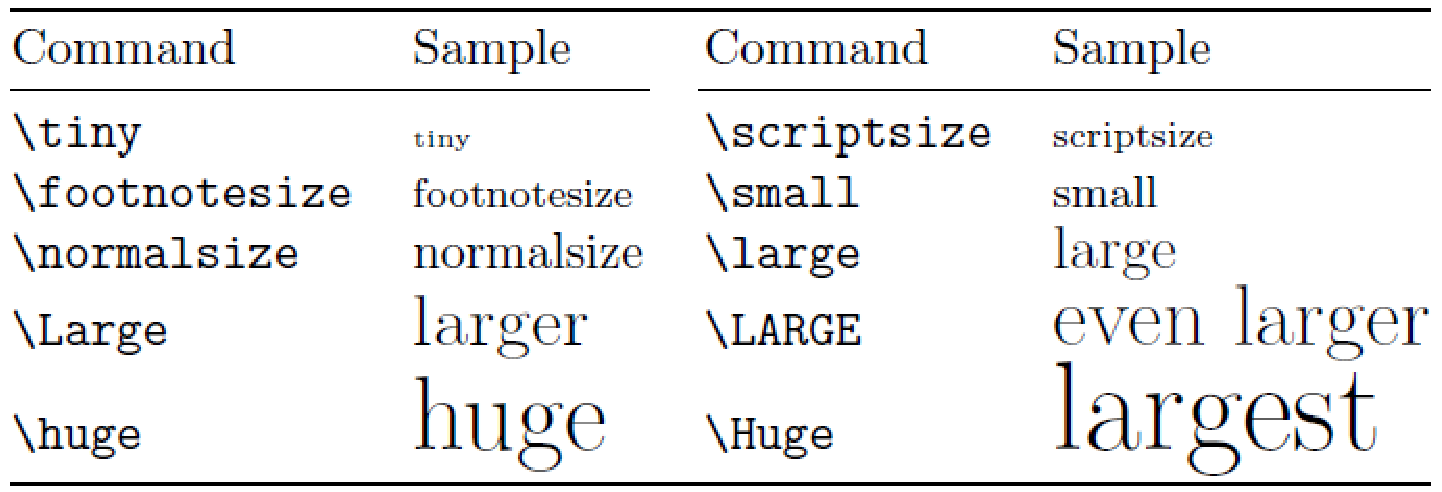
\includegraphics[width=0.7\textwidth]{img/fontsize}
% 	\caption{Exemplo de tamanhos de fonte}
% 	\label{fig:fontsize}
% \end{figure}

% \textbf{Referências dentro do Texto} Partes do texto podem ser referenciadas através do par de comandos \verb|\label| e \verb|\ref|.
%   Por exemplo, podemos inserir uma seção no artigo utilizando o seguinte comando:

% \begin{verbatim}
% \section{Seção principal}\label{sec:prcpal}
% \end{verbatim}

% Vejam que o título da seção é seguido do comando \verb|\label{nome}|.
%   Esta seção pode ser referenciada em qualquer parte do texto, como o exemplo a seguir.

% \begin{verbatim}
% Conforme explicado na Seção \ref{sec:prcpal}, nosso método utiliza...
% \end{verbatim}


% %------------------------------------------------------------------------------
% \section{Outras Dicas}
% %------------------------------------------------------------------------------

% \textbf{Caracteres Especiais} Esses não podem ser usados no texto sem a barra à frente: \# \$ \% \^{ } \& \_ \{ \} \~{ } e \slash .

% \textbf{Comentários} Comentários são precedidos de \% e podem estar em qualquer parte do texto.
%   Lembrando que tudo que estiver após \% será considerado como comentário e ignorado pelo processador.

% \textbf{Incluir Figuras} Incluir figuras no LaTeX é relativamente fácil quando se tem um formato de arquivo pré-definido.
%   or exemplo, neste documento, usa-se apenas figuras do tipo \textit{pdf}, mas também poderia-se usar do tipo \textit{png} (e \textit{jpeg}, mas este tipo não é recomendado).
%   A Tabela \ref{tab:codfig} ilustra as linhas que inserem uma figura no texto. 

% \begin{table}[!htb][ht]
%   \caption{Linhas de código para inserir figura}
% 	\centering
% 	\footnotesize	
% 		\begin{tabular}{l l}
% 	\\	\hline 
% Linha de Código & Explicação \\ \hline 
% \verb|\usepackage{graphicx}| & \textit{inclui pacote gráfico no início do documento} \\
% \verb|\begin{figure}[tb]|    & \textit{inicia figura, define sua posição no texto} \\
% \verb|\centering|            & \textit{centraliza a figura na página}\\
% \verb|\includegraphics[scale=.7]|& \textit{define escala da figura}\\
% \verb|{img/figura}|      & \textit{inclui o arquivo da figura no texto}\\
% \verb|\caption{Legenda}|     & \textit{inclui a legenda da figura}\\
% \verb|\label{fig:ap}|        & \textit{inclui o apelido da figura}\\
% \verb|\end{figure}|          & \textit{termina figura}\\
% 		\hline\end{tabular}
% 	\label{tab:codfig}
% \end{table}

% \textbf{Hifenização} Às vezes aparece uma palavra cuja hifenização, divisão silábica, está errada. Para resolver esse tipo de problema, pode-se recorrer à divisão manual da palavra, acrescentando \verb|\-| entre cada sílaba: \verb|Mi\-re\-lla|. Se, ao invés desta solução, você quiser evitar completamente que suas palavras sejam divididas, acrescente os dois comandos no início do seu documento (ou seja, antes do \\~\textit{begin\{document\}}).

% \begin{verbatim}
%   \hyphenpenalty=5000
%   \tolerance=1000
% \end{verbatim}


% \textbf{BibTeX} Para editar facilmente o BibTeX, pode-se utilizar uma ferramenta própria\footnote{Ferramentas para BibTeX: http://dmoz.org/Computers/Software/Typesetting/TeX/BibTeX}. A minha favorita é o JabRef\footnote{JabRef Editor: http://jabref.sourceforge.net/}, ilustrado na Figure \ref{fig:jabref}, porque:

% \begin{itemize}\addtolength{\itemsep}{-0.5\baselineskip}
% 	\item É de graça;
% 	\item Possui interface gráfica super intuitiva;
% 	\item Permite importar referências de bases clássicas, como ISI, Medline e RIS;
% 	\item Permite exportar para diferentes formatos, inclusive para um banco de dados utilizando SQL;
% 	\item Tem botão para procurar o artigo da respectiva referência e fazer o seu download;
% 	\item Permite adicionar comentários próprios para cada entrada;
% 	\item Pode-ser classificar as referências e criar grupos para as mesmas, e muito muito mais.
% \end{itemize}

% \begin{figure}[tb]
% 	\centering
% 		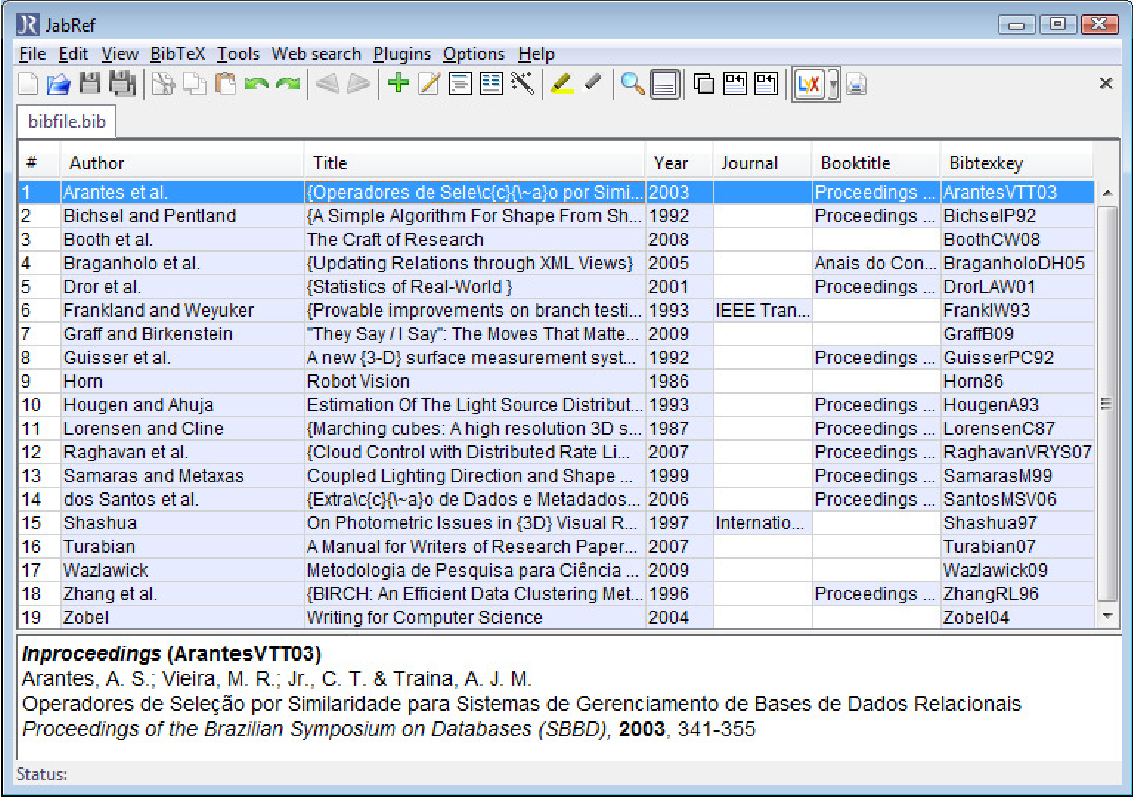
\includegraphics[width=0.98\textwidth]{img/jabref}
% 	\caption{Tela do JabRef para uma versão inicial do arquivo bib deste documento}
% 	\label{fig:jabref}
% \end{figure}

% \textbf{Listas} Listas podem ser definidas com \textit{bullets} ou com números, conforme os exemplos a seguir.

% \begin{verbatim}
% \begin{itemize}
% \item Item 1 com bullet 
% \item Item 2 com bullet 
% \end{itemize}

% \begin{enumerate}
% 	\item Item 1 numerado
% 	\item Item 2 numerado
% \end{enumerate}
% \end{verbatim}

% \textbf{Fontes Coloridas} Para adicionar texto em cores (muito útil para marcar trechos do texto que estão \textit{em trabalho}, deve-se adicionar os pacotes \textit{graphicx} e \textit{color} (usando o comando \verb|\usepackage| e depois utilizar o comando \verb|\textcolor{cor}{texto}| para colorir o \textit{texto} com a \textit{cor} especificada. Por exemplo \verb|\textcolor{blue}{texto em azul}|. Outras cores comuns são \textit{red} e \textit{green}.

% \textbf{Para Economizar Espaço} Existem alguns \textit{dirty tricks}\footnote{Ou seja, eles irão alterar a formatação dada pelo estilo default do texto.} pra economizar espaço, como por exemplo:

% -- \verb|\usepackage{times}| Usa fonte \textit{Times} no lugar da default.

% -- \verb|\usepackage[small,compact]{titlesec}| Modifica o título e os espaços antes/depois dos mesmos.

% -- \verb|\usepackage[small,it]{caption}| Reduz o tamanho das legendas de tabelas e figuras.

% \textbf{WEB} A Web é repleta de páginas e documentos sobre LaTeX. Alguns exemplos incluem:

% \begin{itemize}\addtolength{\itemsep}{-0.5\baselineskip}
%   \item Favorito inglês: \url{http://en.wikibooks.org/wiki/LaTeX/}
%   \item Favorito português: \url{http://linorg.usp.br/CTAN/info/lshort/portuguese/pt-lshort.pdf}
%   \item \url{http://www.mat.ufmg.br/~regi/topicos/intlat.pdf}
%   \item \url{http://www.duke.edu/~hg9/ctex/LaTeXManual.pdf}
%   \item \url{http://minerva.ufpel.tche.br/~campani/cursolatex.pdf}
% 	\item \url{http://www.personal.ceu.hu/tex/words.htm}
% \end{itemize}


% \end{anexosenv}
 % Anexos [OPCIONAL]
\printindex % Índice Remissivo [OPCIONAL]

\end{document}
